\documentclass[]{beamer}
\usepackage[T1]{fontenc}
\usepackage[utf8]{inputenc}
\usepackage{lmodern}
\usepackage[italian]{babel}
\usepackage{mathrsfs}
\usepackage{cancel}

\title{La gravitazione}
\author{\texorpdfstring{Mattia Cozzi\newline\href{mailto:cozzimattia@gmail.com}{\texttt{cozzimattia@gmail.com}}}{Mattia Cozzi}}
\date{a.s.~2023/2024}

%\documentclass[handout]{beamer}     %usare questa classe per generare l'handout
%\usepackage{pgfpages}   %per mostrare più quadri nella stessa pagina
%\pgfpagesuselayout{4 on 1}[a4paper,border shrink=5mm,landscape]
\usetheme{Singapore}
%\useoutertheme[left]{sidebar} %elementi intorno alle diapositive
\setbeamercovered{dynamic} %modifica l'aspetto del testo grigetto delle diapositive future. Argomenti: invisible/transparent/dynamic
\usecolortheme{orchid}
%COLORE PRINCIPALE
\definecolor{marroncino}{RGB}{156, 26, 0} % UBC Blue (primary)
\setbeamercolor{structure}{fg=marroncino} % itemize, enumerate, etc

\theoremstyle{plain}
\newtheorem{teorema}{Teorema}

\usepackage{tikz}
\usepackage{circuitikz}

\usepackage{pgf,pgfplots,graphicx}
\usetikzlibrary{angles,quotes,arrows,shapes,decorations.markings}
\pgfplotsset{compat=1.15}
\usepgfplotslibrary{units,fillbetween} % to add units easily to axis

\newcommand{\fem}{f_{em}}

\def\angolo[#1](#2)(#3:#4:#5)% Syntax: [draw options] (center) (initial angle:final angle:radius)
    { \draw[#1] ($(#2)+({#5*cos(#3)},{#5*sin(#3)})$) arc (#3:#4:#5); }


\begin{document}

\begin{frame}
  \titlepage
\end{frame}





\begin{frame}
\frametitle{Contenuti}
\tableofcontents
\end{frame}


\section{Keplero}


\begin{frame}
\frametitle{Modello cosmologico}
\begin{columns}
\begin{column}{0.2\textwidth}
\visible<1->{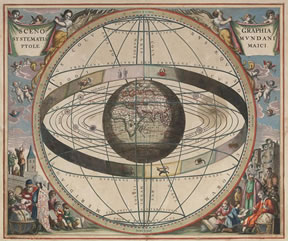
\includegraphics[width=\columnwidth]{img/tolomeo.jpg}}
~
\visible<2->{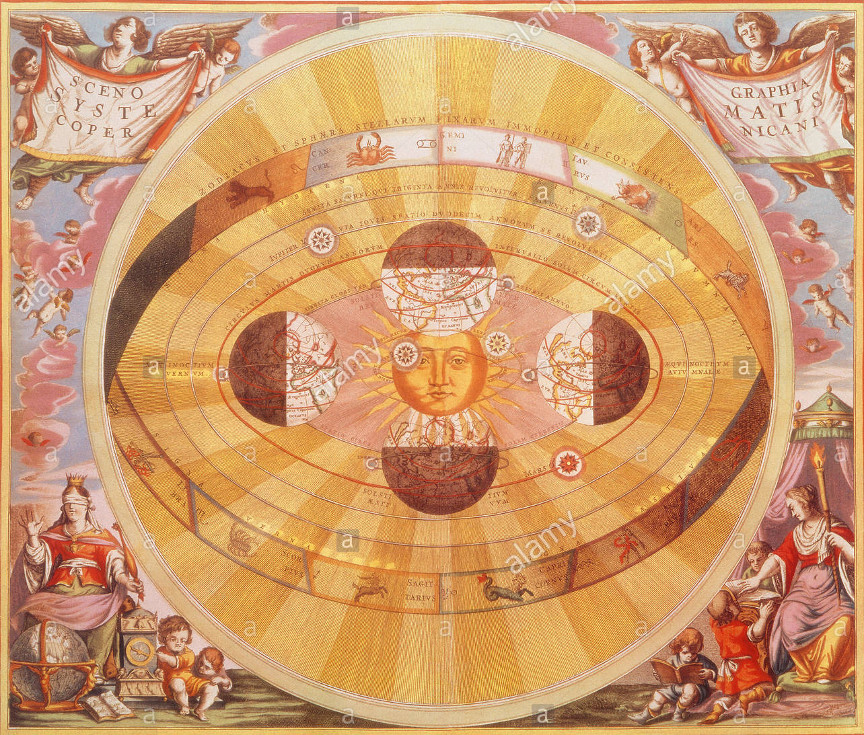
\includegraphics[width=\columnwidth]{img/copernico.jpg}}
~
\visible<3->{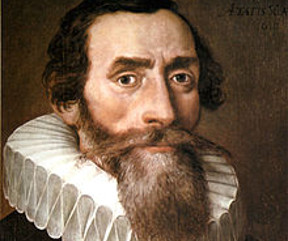
\includegraphics[width=\columnwidth]{img/keplero.jpg}}
\end{column}
\begin{column}{0.6\textwidth}
\begin{itemize}
\item<1-> Tolomeo (150, \emph{Almagesto}) propone un modello \alert<1>{geocentrico} con orbite circolari;
\item<2-> Niccolò Copernico (1543, \emph{De Revolutionibus Orbium Coelestium}) propone un modello \alert<2>{eliocentrico};
\item<3-> Johannes Kepler enuncia le sue \alert<3>{leggi} (1609, \emph{Astronomia Nova});
\item<4-> Isaac Newton propone la \alert<4>{gravitazione universale} (1687, \emph{Philosophiae Naturalis Principia Mathematica}).
\end{itemize}
\end{column}
\end{columns}
\end{frame}

\begin{frame}
\frametitle{Il modello eliocentrico}
Il modello di Copernico fu concepito per ridurre la complessità dei calcoli necessari a predire le posizioni dei pianeti.

~

Prevedeva il Sole al centro ed i pianeti in orbita intorno ad esso, secondo \alert{traiettorie circolari}.

~

Il modello di Copernico non era però perfetto: i calcoli non erano in accordo con le osservazioni astronomiche (molto precise quelle di Tycho Brahe, fine XVI secolo).
\end{frame}

\begin{frame}
\frametitle{Keplero}
Keplero risolse i problemi del modello copernicano proponendo \alert{orbite ellittiche} anziché circolari.
\begin{figure}
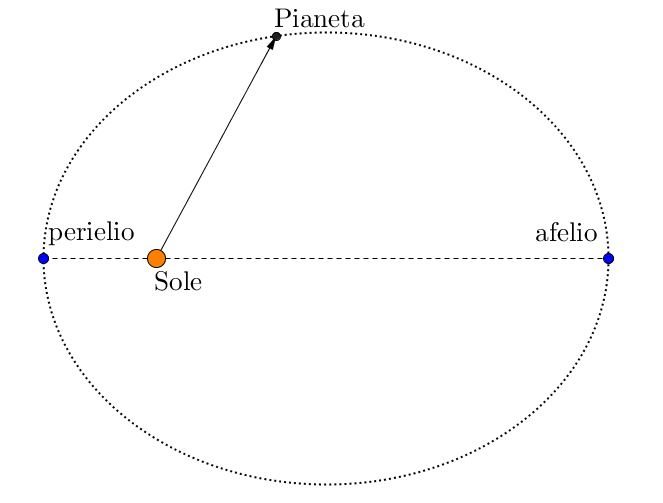
\includegraphics[width=.5\columnwidth]{img/orbitaellittica.jpg}
\end{figure}

\begin{center}
\href{gif/ellisse.gif}{\beamergotobutton{Video: Generazione di un'ellisse}}
\end{center}
\end{frame}


\begin{frame}
\frametitle{La prima legge}
\begin{block}{Prima legge di Keplero}
Le orbite descritte dai pianeti attorno al Sole sono ellissi di cui il Sole occupa uno dei due fuochi.
\end{block}
\begin{center}
\href{gif/keplero1.gif}{\beamergotobutton{GIF: Prima legge}}
\end{center}\pause


Generalmente, l'eccentricità dell'orbita dei pianeti è molto bassa ($ e_{Terra} = 0,017 $) e possiamo spesso approssimare l'orbita come circolare (tuttavia $ e_{Plutone} = 0,244 $).
\end{frame}


\begin{frame}
\frametitle{La seconda legge}
\begin{block}{Seconda legge di Keplero}
Il raggio vettore che va dal Sole ad un pianeta spazza aree uguali in intervalli di tempo uguali.
\end{block}
\begin{figure}
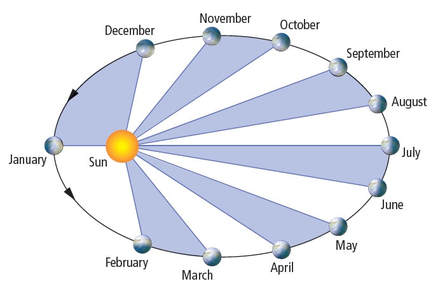
\includegraphics[width=.5\columnwidth]{img/keplero2.jpg}

\href{gif/keplero2.gif}{\beamergotobutton{GIF: Seconda legge}}
\end{figure}\pause
Il pianeta risulta più veloce al perielio e più lento all'afelio.
\end{frame}



\begin{frame}
\frametitle{La terza legge}
\begin{block}{Terza legge di Keplero}
Il rapporto tra il cubo del semiasse maggiore dell'orbita e il quadrato del periodo di rivoluzione è lo stesso per tutti i pianeti.
\begin{center}
\colorbox{marroncino!30}{$ \dfrac{a^3}{T^2}=k $}
\end{center}
\end{block}\pause

~

Ne risulta che più un pianeta è distante dal Sole, maggiore è il suo periodo di rivoluzione: 
\begin{itemize}
  \item $ a_{Terra} = 1,5 \times 10^{11} \, m $ e $ T_{Terra} = 1 \, anno $;\pause
  \item $ a_{Plutone} = 5,9 \times 10^{12} \, m = $ e $ T_{Plutone} = 249,7 \, anni $.
\end{itemize}
\begin{center}
\href{gif/keplero3.gif}{\beamergotobutton{GIF: Terza legge}}
\end{center}
\end{frame}





\section{Gravitazione universale}






\begin{frame}
\frametitle{Leggi descrittive e leggi causali}
Le leggi di Keplero descrivono ottimamente il moto dei pianeti intorno al Sole, ma non spiegano il \emph{motivo} di tali moti.\pause

~

Newton propose una forza, la \alert{forza di gravità}, per cui due corpi dotati di massa si attraggono.\pause

~

La stessa forza che fa cadere a terra gli oggetti, tiene in orbita i pianeti e i loro satelliti.
\end{frame}



\begin{frame}
\frametitle{La gravitazione universale (1)}
\begin{block}{Legge di gravitazione universale}
La forza di attrazione gravitazionale tra due corpi puntiformi di massa $ m_1 $ e $ m_2 $ a distanza $ r $ è diretta lungo la linea che congiunge i due corpi e ha modulo:
\begin{center}
\colorbox{marroncino!30}{$ F = G \,  \dfrac{m_1 \, m_2}{r^2} $}
\end{center}
$ G = 6,67 \times 10^{-11} \, \frac{Nm^2}{kg^2}$ =  cost.~di gravitazione universale
\end{block}
\end{frame}

\begin{frame}
\frametitle{La gravitazione universale (2)}
\begin{columns}
\begin{column}{0.3\textwidth}
\begin{center}
\colorbox{marroncino!30}{$ F = G \,  \dfrac{m_1 \, m_2}{r^2} $}
\end{center}
\end{column}
\begin{column}{0.5\textwidth}
\begin{figure}
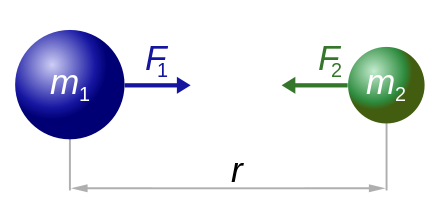
\includegraphics[width=\columnwidth]{img/gravitazione.png}
\end{figure}
\end{column}
\end{columns}\pause

Notiamo che:
\begin{itemize}
  \item se una delle masse raddoppia, la forza di attrazione raddoppia;\pause
  \item se la distanza raddoppia, le forza di attrazione diventa quattro volte meno intensa (non ``sentiamo'' la gravità delle stelle!).
\end{itemize}
\end{frame}



\begin{frame}
\frametitle{Esercizio}
\begin{exampleblock}{Gravitazione di un satellite artificiale}
  \small{Un satellite di diametro trascurabile orbita intorno alla Terra alla distanza di $ 500 \, km $ dalla superficie terrestre e risente di una forza di $ 3,50 \times 10^{6} \, N $. La massa della Terra vale $ 5,976 \times 10^{24} \, kg $. Trattiamo il problema come se le masse dei corpi fossero tutte concentrate nei loro centri. 

  Quanto vale la massa del satellite?\hspace*{\fill}[$ 4,16 \times 10^{5} \, kg $]}
\end{exampleblock}\pause

~

Ricorda che la distanza tra i due centri di massa è pari alla somma tra il raggio terrestre e l'altitudine dell'orbita.
\end{frame}



\begin{frame}
\frametitle{Gravitazione universale e leggi di Keplero}
Le tre leggi di Keplero possono essere dedotte matematicamente dalla legge di gravitazione universale.\pause

~

La legge di gravitazione universale motiva quindi le tre leggi descrittive di Keplero.
\end{frame}



\end{document}
